\documentclass[aspectratio=169,9pt,t]{beamer}
\usefonttheme{professionalfonts}
\usefonttheme{serif}
\usepackage{amsmath}
\usepackage{unicode-math}
\setmainfont{Latin Modern Roman}[Ligatures=TeX]
\setsansfont{Latin Modern Roman}[Ligatures=TeX]
\setmonofont{Latin Modern Mono}[Scale=0.9]
\setmathfont{Latin Modern Math}
\usepackage{kr}
\usepackage{booktabs,tabularx,array,ragged2e,graphicx,tikz,appendixnumberbeamer}
\usetikzlibrary{positioning,calc}

%---------------------------------------------------------------- 색·크기
\definecolor{ink}{HTML}{1A1A1A}
\definecolor{navy}{HTML}{1F3A5F}
\definecolor{crim}{HTML}{9B2335}
\definecolor{mute}{HTML}{5A626C}
\definecolor{hair}{HTML}{B8BDC4}
\definecolor{wash}{HTML}{F1F4F8}
\setbeamercolor{normal text}{fg=ink,bg=white}
\setbeamercolor{frametitle}{fg=ink,bg=white}
\setbeamercolor{structure}{fg=navy}
\setbeamercolor{alerted text}{fg=crim}
\setbeamersize{text margin left=11mm,text margin right=11mm}
\setbeamertemplate{navigation symbols}{}
\linespread{1.16}
\frenchspacing

%---------------------------------------------------------------- 제목줄·바닥줄
\setbeamerfont{frametitle}{size=\large}
\setbeamertemplate{frametitle}{%
  \vspace{2.6mm}%
  {\fontsize{7.6}{9.5}\selectfont\bfseries\color{navy}\insertsectionhead\strut\par}%
  \vspace{0.3mm}%
  {\fontsize{16}{19}\bfseries\selectfont\color{ink}\insertframetitle\par}%
  \vspace{1.6mm}%
  {\color{ink}\hrule height 0.6pt}%
  \vspace{2.4mm}}
\setbeamertemplate{footline}{%
  \leavevmode\hspace{11mm}%
  \begin{minipage}{\dimexpr\paperwidth-22mm\relax}
  {\fontsize{7}{9}\selectfont\color{mute}%
   박찬진\quad|\quad 실행되지 않는 위협의 발표효과\hfill\insertframenumber\,/\,\inserttotalframenumber}
  \end{minipage}\vspace{2.8mm}}

%---------------------------------------------------------------- 목록
\setbeamertemplate{itemize item}{\raisebox{0.28ex}{\tiny\color{navy}$\blacksquare$}}
\setbeamertemplate{itemize subitem}{\color{mute}--}
\setlength{\leftmargini}{1.25em}
\setlength{\leftmarginii}{1.2em}
\setbeamerfont{itemize/enumerate subbody}{size=\small}
\let\olditemize\itemize
\renewcommand{\itemize}{\olditemize\setlength{\itemsep}{0.42em}}

%---------------------------------------------------------------- 도구
\newcommand{\msg}[1]{{\fontsize{11.5}{15}\selectfont\bfseries\color{navy}\RaggedRight #1\par}\vspace{2.0mm}}
\newcommand{\key}[1]{{\bfseries\color{crim}#1}}
\newcommand{\takeaway}[1]{%
  \par\vfill
  \noindent\colorbox{wash}{\begin{minipage}[c]{\dimexpr\linewidth-2\fboxsep\relax}\vspace{0.5mm}\hspace{1.5mm}{\color{crim}\bfseries$\rightarrow$}\hspace{1.5mm}%
  \begin{minipage}[c]{\dimexpr\linewidth-9mm\relax}\fontsize{8.6}{11}\selectfont\RaggedRight #1\end{minipage}\vspace{0.5mm}\end{minipage}}\par\vspace{0.8mm}}
\newcommand{\src}[1]{\par\vspace{0.8mm}{\fontsize{6.8}{8.6}\selectfont\color{mute}\RaggedRight #1\par}}
\newcommand{\lab}[1]{{\fontsize{8.4}{10.5}\selectfont\bfseries\color{crim}#1}}
\newcommand{\hyp}[1]{\textbf{H#1}}
\newcommand{\Bcit}{B^{\mathrm{cit}}}
\newcommand{\Bfam}{B^{\mathrm{fam}}}
\newcommand{\pp}{\%p}
\newcolumntype{L}[1]{>{\RaggedRight\arraybackslash\hspace{0pt}}p{#1}}
\newcolumntype{Y}{>{\RaggedRight\arraybackslash\hspace{0pt}}X}
\newcolumntype{R}[1]{>{\raggedleft\arraybackslash}p{#1}}
\renewcommand{\arraystretch}{1.3}
\setlength{\heavyrulewidth}{0.8pt}\setlength{\lightrulewidth}{0.4pt}
\newcommand{\tf}{\fontsize{8.2}{10.4}\selectfont}
\newcommand{\tfs}{\fontsize{7.5}{9.4}\selectfont\renewcommand{\arraystretch}{1.18}}

\title{실행되지 않는 위협의 발표효과}

\newcommand{\todo}[1]{\par\vspace{2mm}\noindent\fcolorbox{crim}{white}{\begin{minipage}{\dimexpr\linewidth-4mm\relax}\small\color{crim}\textbf{자료 대기}\quad\color{ink}#1\end{minipage}}\par}
\begin{document}

{
\setbeamertemplate{footline}{}
\begin{frame}[noframenumbering]
\vspace{14mm}
{\fontsize{8.5}{11}\selectfont\bfseries\color{navy} 학술발표\quad|\quad 2026년 11월\par}
\vspace{3mm}
{\fontsize{25}{31}\selectfont\bfseries 실행되지 않는 위협의 발표효과\par}
\vspace{3.5mm}
{\fontsize{13}{17}\selectfont 관세 위협과 수출통제 예고에 대한 고빈도 사건연구, 2025--2026\par}
\vspace{6mm}
{\color{ink}\hrule height 0.5pt}
\vspace{6mm}
{\large 박찬진\par}
\vspace{1.5mm}
{\small\color{mute} 2026년 11월 15일\quad|\quad 작업본\par}
\vfill
{\footnotesize\color{mute}\linespread{1.15}\selectfont 사건 목록과 분석 계획은 가격 자료를 보기 전에 고정했다. 탐색적 연구이며 표본이 작다.\par}
\vspace{6mm}
\end{frame}
}

%================================================================
\section{발표효과}

\begin{frame}{PMCCF: 매입 없는 발표효과}
\msg{한 푼도 쓰지 않은 정책이 시장을 되돌렸다}
\begin{columns}[T,onlytextwidth]
\begin{column}{0.53\textwidth}
\lab{2020년 3월, 미국 회사채 시장}
\begin{itemize}
\item 3월 23일 연준이 회사채 매입기구 두 개(PMCCF, SMCCF)를 \textbf{발표}
\item 발표 시점에 투자등급 회사채 가격이 약 7\% 상승, 다른 자산은 거의 무반응
\item 실제 매입은 한참 뒤: SMCCF 5월 12일, PMCCF 6월 29일 개시
\end{itemize}
\end{column}
\begin{column}{0.42\textwidth}
\lab{실제로 쓴 돈}\par\vspace{1.5mm}
\begingroup\tf
\begin{tabularx}{\linewidth}{@{}Yr@{}}
\toprule
기구 & 최대 이용액\\
\midrule
SMCCF (유통시장) & 141억 달러\\
PMCCF (발행시장) & \textbf{0달러}\\
\bottomrule
\end{tabularx}\endgroup
\vspace{2.5mm}
{\small\RaggedRight PMCCF는 한 건도 매입하지 않고 종료됐다. 시장을 움직인 것은 매입이 아니라 \textbf{매입하겠다는 말}이었다.\par}
\end{column}
\end{columns}
\takeaway{발표만으로 가격이 움직이려면 조건이 하나 있다. 시장이 그 말을 \textbf{믿어야} 한다.}
\end{frame}

\begin{frame}{발표효과 문헌}
\msg{발표가 가격을 움직인다는 증거는 많다. 발표자는 늘 약속을 지키는 기관이었다}
\begingroup\tfs
\begin{tabularx}{\textwidth}{@{}L{0.2\textwidth}L{0.34\textwidth}Y@{}}
\toprule
영역 & 발표 & 연구가 보인 것\\
\midrule
양적완화 & 2008--2010년 연준 자산매입 발표 & 매입 전, 발표일에 장기금리 하락 (Krishnamurthy \& Vissing-Jorgensen 2011)\\
포워드 가이던스 & FOMC 성명의 문구 & 금리 결정과 별개로 '미래 경로에 대한 말'이 가격을 움직임 (Gürkaynak et al. 2005)\\
유로 위기 & 2012년 ``whatever it takes''와 OMT & 발동된 적 없는 OMT가 남유럽 국채금리를 낮춤 (Altavilla et al. 2016)\\
코로나 위기 & 2020년 회사채 매입기구 & 발표 시점에 스프레드 축소, PMCCF 매입 0 (Haddad et al. 2021)\\
무역정책 & 2018--2019년 관세 발표 & 발표일 주가 하락과 이후 실물 성과 (Amiti et al.)\\
\bottomrule
\end{tabularx}\endgroup
\end{frame}

\begin{frame}{관세 위협의 실행 실적}
\msg{강화 위협 33건 중 21건이 실행되지 않았다}
\begin{columns}[c,onlytextwidth]
\begin{column}{0.56\textwidth}
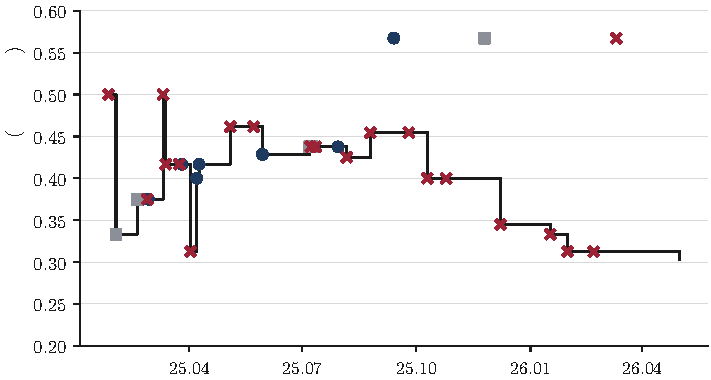
\includegraphics[width=\linewidth]{fig/cred_path.pdf}
\end{column}
\begin{column}{0.4\textwidth}
\begingroup\tf
\begin{tabularx}{\linewidth}{@{}Yr@{}}
\toprule
강화 위협 33건의 결과 & \\
\midrule
실행 & 7\\
부분 실행 & 4\\
미실행 & 21\\
미확정 & 1\\
\bottomrule
\end{tabularx}\endgroup
\vspace{2mm}
{\small\RaggedRight 실행률은 2025년 내내 0.40--0.46, 2026년에 0.31.\par}
\end{column}
\end{columns}
\end{frame}

\begin{frame}{연구 질문과 예측}
\msg{실행되지 않는 위협이 반복될 때, 위협의 발표효과는 어떻게 되는가}
\begin{itemize}
\item \textbf{왜 중요한가}\; 위협은 실행 비용 없이 협상력을 얻는 수단이다. 시장이 믿지 않으면 그 수단은 사라진다
\end{itemize}
\vspace{1mm}
\lab{세 가지 예측 (단순 학습 모형: 반응 $\approx \Delta p \times L$)}\par\vspace{1mm}
\begingroup\tf
\begin{tabularx}{\textwidth}{@{}lL{0.38\textwidth}Y@{}}
\toprule
 & 시장이 위협을 덜 믿으면 & 구분해 주는 것\\
\midrule
P1 & 위협 발표 시점의 반응이 작다 & 이것만으로는 '관세 뉴스에 무뎌진 것'과 구분되지 않음\\
P2 & 예정 발효 시점의 반응이 \textbf{크다} & 발표를 안 믿었으면 발효가 새 정보. 무뎌진 것이라면 여기도 작아야 함\\
P3 & 철회·완화 시점의 반응이 작다 & 처음에 덜 반영됐으면 되돌릴 것도 적음\\
\bottomrule
\end{tabularx}\endgroup
\takeaway{이 질문에 오기까지 두 번 실패했다. 그 과정이 지금의 방법을 정했다.}
\end{frame}

%================================================================
\section{첫 시도}

\begin{frame}{2018년 수출통제 예고와 특허}
\msg{원래 질문: 예고만으로 중국의 연구배분이 바뀌었는가}
\begin{columns}[T,onlytextwidth]
\begin{column}{0.5\textwidth}
\lab{원래 질문}
\begin{itemize}
\item 2018년 11월 미국이 신흥기술 수출통제를 \textbf{예고}(ANPRM)
\end{itemize}
\vspace{1mm}
\lab{설계}
\begin{itemize}
\item 18기술 $\times$ 5국 $\times$ 120개월 특허 패널
\item 지목 기술 대 비지목 기술, 사전 미국 의존도가 높을수록 반응이 큰지
\end{itemize}
\end{column}
\begin{column}{0.45\textwidth}
\lab{모형이 말해 준 것}
\[\frac{dI^{*}}{dp}=-\frac{D\,R_{Ia}}{C''-R_{II}},\qquad \frac{dV}{dp}<0\]
\begin{itemize}
\item 규제 확률 $p$가 오르면 기업가치 $V$는 항상 하락
\item 자체 연구 $I^{*}$는 대체재면 증가, 보완재면 감소
\item \textbf{주가만으로는 연구의 방향을 알 수 없다}
\end{itemize}
\end{column}
\end{columns}
\end{frame}

\begin{frame}{식별 실패 1: 공통 지지 영역}
\msg{비교할 기술이 없었다}
\begin{columns}[c,onlytextwidth]
\begin{column}{0.54\textwidth}
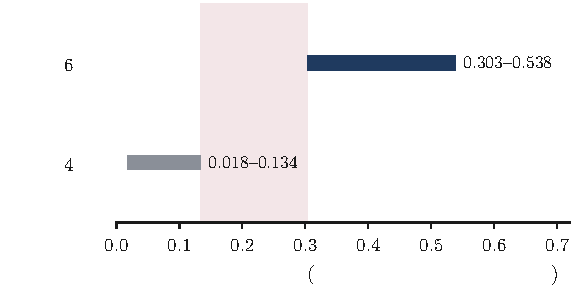
\includegraphics[width=\linewidth]{fig/dose_ranges.pdf}
\end{column}
\begin{column}{0.42\textwidth}
\begin{itemize}
\item 지목 기술: AI·음성인식·적층제조 등
\item 비지목 기술: 성형·절삭·연삭
\item 미국 의존도 범위가 \textbf{한 곳도 겹치지 않는다}
\item 대체 지표로 겹치는 구간을 만들면 지목 2, 비지목 3단위만 남는다
\end{itemize}
\end{column}
\end{columns}
\takeaway{``같은 의존도의 지목 기술과 비지목 기술''이라는 비교 자체가 자료에 없었다. 지목된 기술은 애초에 다른 종류의 기술이었다.}
\end{frame}

\begin{frame}{식별 실패 2: 가짜 시점 검정}
\msg{아무 일도 없던 해에 ``효과''가 더 컸다}
\begin{columns}[c,onlytextwidth]
\begin{column}{0.52\textwidth}
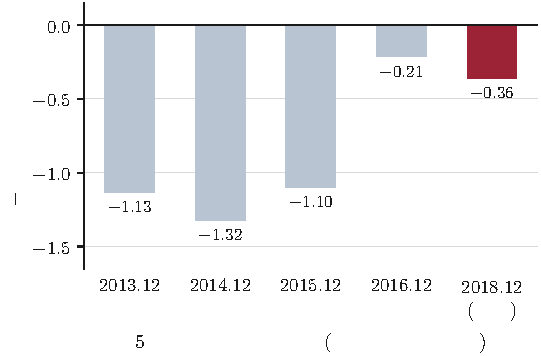
\includegraphics[width=\linewidth]{fig/fake_windows.pdf}
\end{column}
\begin{column}{0.44\textwidth}
\begin{itemize}
\item 실제 창(2018.12--2019.4)의 추정치: $-0.359$
\item 신호가 없던 2013--2015년 같은 달 창: $-1.1$에서 $-1.3$
\item 의존도를 4,999번 재배정해도 실제 추정치는 이례적이지 않았다
\end{itemize}
\end{column}
\end{columns}
\end{frame}

\begin{frame}{식별 실패 3: 사전 추세}
\msg{신호 이전부터 경로가 흔들렸다}
\begin{columns}[c,onlytextwidth]
\begin{column}{0.56\textwidth}
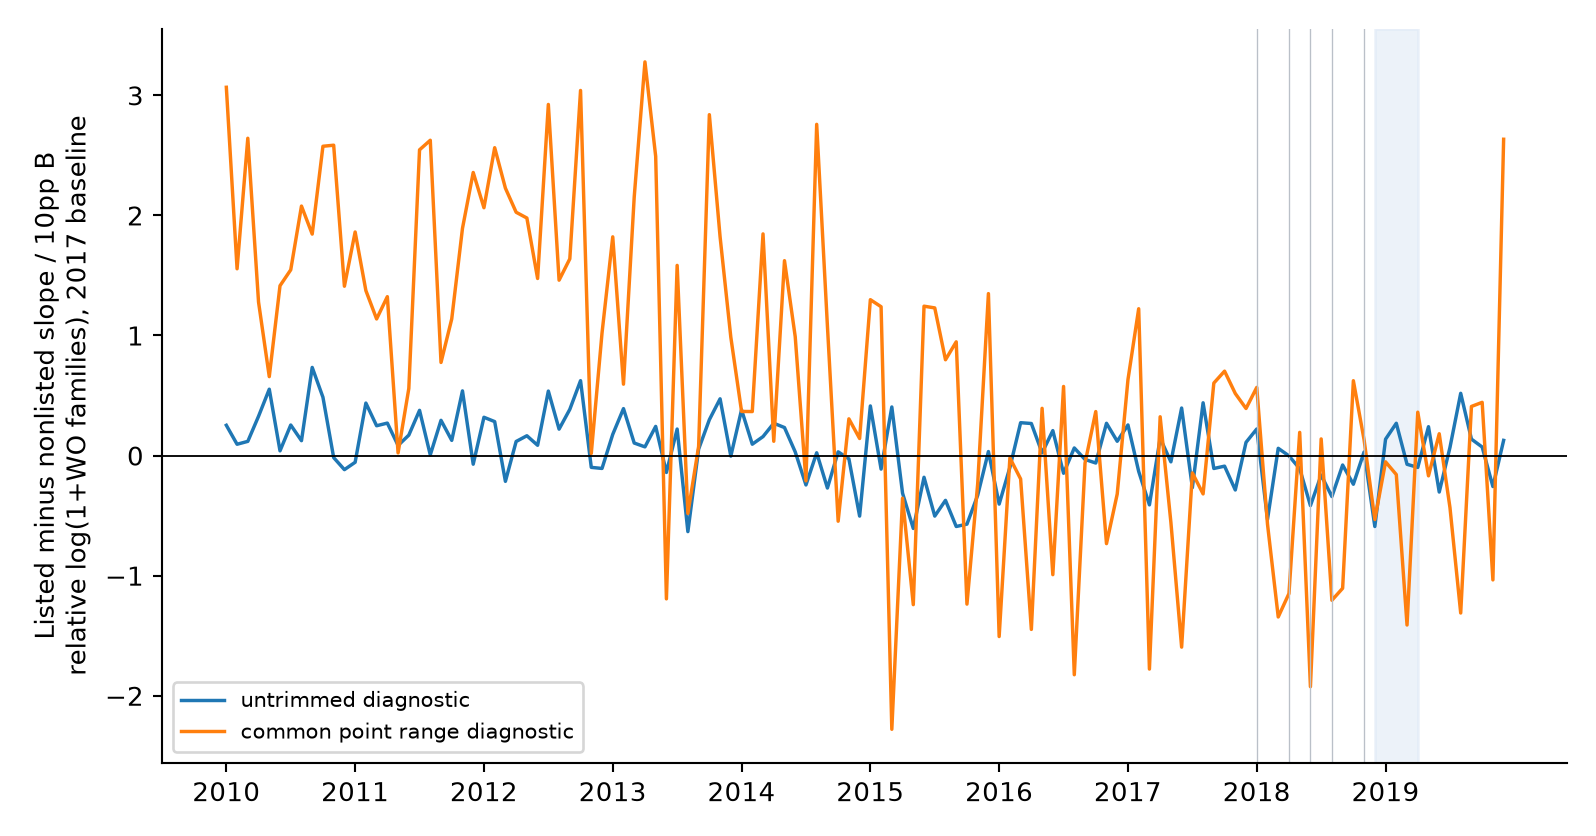
\includegraphics[width=\linewidth]{fig/fig4_theta_orig.png}
\end{column}
\begin{column}{0.4\textwidth}
\begin{itemize}
\item 2010--2017년 사이 차등 기울기가 $+3$에서 $-2$까지 움직인다
\item 2018년 신호(세로선) 전후로 달라진 패턴이 보이지 않는다
\item 5개월 창으로 특허 출원의 반응을 잡기에는 연구에서 출원까지의 시차도 길다
\end{itemize}
\end{column}
\end{columns}
\takeaway{판정: 이 설계로는 연구배분의 인과효과를 말할 수 없다. 효과가 없다는 증거도 아니다.}
\end{frame}

\begin{frame}{첫 시도의 교훈}
\begin{columns}[T,onlytextwidth]
\begin{column}{0.48\textwidth}
\lab{버린 것}
\begin{itemize}
\item 특허로 연구배분을 재는 설계
\item 특허 인용 비중을 '미국 의존도'로 쓰는 지표
\item ``기술 대응''이라는 결과 변수
\end{itemize}
\end{column}
\begin{column}{0.48\textwidth}
\lab{남긴 것}
\begin{itemize}
\item 신호는 한 번에 오지 않는다: 보고서, 입법, 예고, 시행이 따로 도착한다
\item \textbf{예고와 시행을 구분}해야 한다
\item 가짜 시점·재배정으로 설계를 먼저 깨 보는 절차
\end{itemize}
\end{column}
\end{columns}
\takeaway{질문을 줄였다. ``예고가 연구를 바꿨는가'' 대신, 그 앞 단계인 ``예고가 정보로서 시장에 도착했는가''부터 보기로 했다.}
\end{frame}

%================================================================
\section{두 번째 시도}

\begin{frame}{단일 사건: 2025년 10월 10일}
\msg{위협 게시 후 한 시간에 중국 ADR $-4\%$}
\begin{columns}[c,onlytextwidth]
\begin{column}{0.58\textwidth}
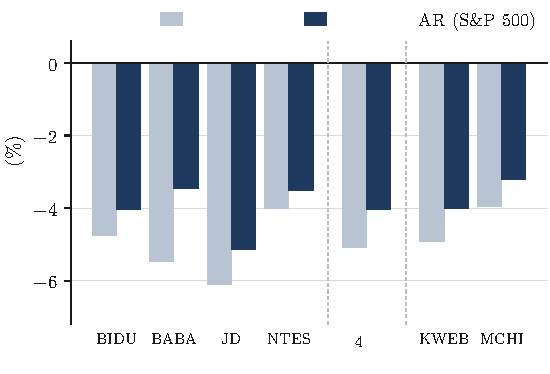
\includegraphics[width=0.9\linewidth]{fig/s_fig_ar.pdf}
\end{column}
\begin{column}{0.38\textwidth}
\begin{itemize}
\item 10:57 ET 대통령의 대중 관세 인상 위협 게시
\item 그 시각을 포함한 한 시간에 중국 ADR 4사 $-5.09\%$, 시장조정 후 $-4.03\%$
\item 과거 59거래일 같은 시각 중 최대
\end{itemize}
\end{column}
\end{columns}
\end{frame}

\begin{frame}{교훈 1: 게시 시각}
\msg{시각이 틀리면 원인이 바뀐다}
\begin{columns}[c,onlytextwidth]
\begin{column}{0.58\textwidth}
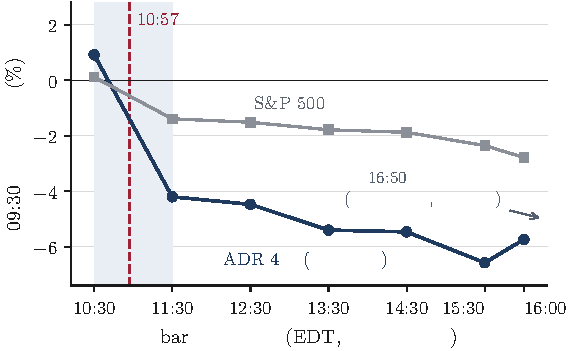
\includegraphics[width=\linewidth]{fig/oct10_path.pdf}
\end{column}
\begin{column}{0.38\textwidth}
\begin{itemize}
\item 그날 보도의 제목은 ``100\% 관세와 소프트웨어 수출통제''
\item 그 구체적 예고는 16:50, \textbf{장 마감 후}
\item 정규장 하락은 10:57의 선행 위협에 대한 반응이다
\item 일별 자료로는 둘을 구분할 수 없다
\end{itemize}
\end{column}
\end{columns}
\end{frame}

\begin{frame}{교훈 2: 외적 타당성}
\msg{사건 하나로는 아무것도 일반화할 수 없다}
\begin{columns}[T,onlytextwidth]
\begin{column}{0.48\textwidth}
\lab{한계}
\begin{itemize}
\item 사건 1개, 기업 4개(목적표본)
\item 중국 ETF를 기준으로 하면 상대 반응이 $+2.0\%$: 기술 특이 반응이 아니라 중국 전체의 위험 재평가
\item 의존도 기울기는 기업 하나를 빼면 부호가 바뀜
\end{itemize}
\end{column}
\begin{column}{0.48\textwidth}
\lab{그리고 그 위협의 결말}
\begin{itemize}
\item 10월 12일(일) 완화성 게시
\item 10월 13일 ADR 4사 $+2.48\%$
\item 10월 30일 합의, 100\% 관세는 1년 연기
\end{itemize}
\vspace{1mm}
{\small\RaggedRight \textbf{결국 실행되지 않았다.} 시장은 $-4\%$를 냈지만 위협은 3주 만에 사라졌다.\par}
\end{column}
\end{columns}
\takeaway{여기서 원래 하고 싶던 질문으로 돌아왔다. 이런 일이 수십 번 반복됐다면, 시장은 그 기록을 가격에 반영하고 있었는가.}
\end{frame}

%================================================================
\section{현재 설계}

\begin{frame}{선행연구와의 차이}
\msg{위협과 시행의 구분, 실행 여부에 따른 반응은 비어 있다}
\begingroup\tf
\begin{tabularx}{\textwidth}{@{}L{0.27\textwidth}L{0.36\textwidth}Y@{}}
\toprule
연구 & 한 것 & 하지 않은 것\\
\midrule
Kalemli-Özcan, Soylu \& Yildirim (2026) & 2025.1--2026.5 관세 발언 전수 DB(TiRADE), 시각 확인 319건, 블룸버그 분 단위로 환율·주가 반응 & 위협과 시행의 구분, 시간에 따른 반응 변화, 과거 미실행 기록의 영향, 예측시장\\
Merendino \& Monacelli (2026) & 분기 VAR와 '관세 지속성에 대한 학습' 모형 & 사건 단위 검정\\
\bottomrule
\end{tabularx}\endgroup
\vspace{2mm}
\begin{itemize}
\item 본 연구의 자리: 사건별 \textbf{실행 여부}를 코딩하고, 발표·발효·철회 세 시점의 반응을 함께 본다
\item 사건 수와 자료 품질은 TiRADE에 미치지 못한다 (무료 자료, 41건)
\end{itemize}
\end{frame}

\begin{frame}{사건 패널}
\msg{57건을 가격을 보기 전에 고정했다}
\begingroup\tfs
\begin{tabularx}{\textwidth}{@{}L{0.2\textwidth}rL{0.3\textwidth}Y@{}}
\toprule
유형 & 건수 & 예 & 시각\\
\midrule
강화 위협·발표 & 33 & EU 50\% (2025.5.23), 그린란드 관련 유럽 8국 (2026.1.17) & 21건 게시 시각 확인, 12건 날짜만\\
완화·철회 & 13 & 상호관세 90일 유예 (2025.4.9), EU 시한 연기 (5.25) & 9건 확인, 4건 날짜만\\
예정 발효 & 11 & 캐나다·멕시코 25\% (2025.3.4), 122조 10\% (2026.2.24) & 발효 시각 00:01 ET\\
\bottomrule
\end{tabularx}\endgroup
\vspace{2mm}
\lab{결과 코딩 규칙 (가격과 무관)}
\begin{itemize}
\item 시한이 있는 위협: 시한에 위협한 세율이 발효 중이면 실행, 줄어서 발효면 부분 실행, 아니면 미실행
\item 시한이 없는 위협: 명시적 철회가 없으면 90일 뒤 미실행으로 확정
\end{itemize}
\end{frame}

\begin{frame}{반응의 측정}
\msg{분 단위 가격을 같은 시각의 비사건 창으로 표준화한다}
\begin{columns}[T,onlytextwidth]
\begin{column}{0.48\textwidth}
\lab{결과 변수}
\begin{itemize}
\item 시장 전체: S\&P 500 (주가 하락 $=+$)
\item 대상국 통화: 달러 대비 약세 $=+$
\item 주 창: 게시 5분 전부터 30분 후
\item 시장이 닫힌 시각의 게시는 재개 후 30분
\end{itemize}
\vspace{1mm}
\lab{표준화}
\begin{itemize}
\item 같은 요일·같은 시각의 비사건 창 60개의 표준편차로 나눈 $z$
\end{itemize}
\end{column}
\begin{column}{0.48\textwidth}
\lab{자료 (전부 무료 공개)}\par\vspace{1mm}
\begingroup\tfs
\begin{tabularx}{\linewidth}{@{}L{0.36\linewidth}Y@{}}
\toprule
Dukascopy & 통화 13종·지수 CFD, 1분봉, 2025.1--\\
Yahoo Finance & 선물·ETF·통화 79종, 시간봉(최근 730일)·일봉\\
Polymarket, Kalshi & 관세 관련 계약의 가격 이력\\
APP, 관보 & 게시 시각, 발효일\\
\bottomrule
\end{tabularx}\endgroup
\end{column}
\end{columns}
\end{frame}

\begin{frame}{검정 설계}
\msg{사건 수에 맞는 질문만 던진다}
\begin{columns}[T,onlytextwidth]
\begin{column}{0.56\textwidth}
\begingroup\tf
\begin{tabularx}{\linewidth}{@{}lY@{}}
\toprule
T1 & 강화 위협의 평균 반응이 0보다 큰가, 전반과 후반이 다른가\\
T2 & 사후에 실행된 위협과 아닌 위협의 \textbf{발표 시점} 반응이 다른가\\
T3 & 예정 발효 시점에 반응이 있는가, 발표 시점보다 큰가\\
T4 & 완화·철회의 평균 반응이 음인가, 전반과 후반이 다른가\\
\bottomrule
\end{tabularx}\endgroup
\vspace{1.5mm}
{\small\RaggedRight 추론은 placebo 분포와 순열 검정. 강건성 14종(창 길이, 실행률 정의, 4월 초 제외 등)을 전부 보고한다.\par}
\end{column}
\begin{column}{0.4\textwidth}
\lab{왜 기울기 회귀를 주 검정에서 뺐나}
\begin{itemize}
\item 실행률이 0.29--0.50에서만 움직인다
\item 합성 자료로 점검하니 사건 20건으로는 기울기를 검출할 수 없었다
\item 두 집단 평균 차이는 표준오차 0.3--0.45 $z$로 검출 가능
\end{itemize}
\end{column}
\end{columns}
\end{frame}

%================================================================
\section{결과}

\begin{frame}{결과 1: 강화 위협의 평균 반응}
\msg{위협은 여전히 시장을 움직인다. 다만 크기는 작다}
\begin{columns}[c,onlytextwidth]
\begin{column}{0.58\textwidth}
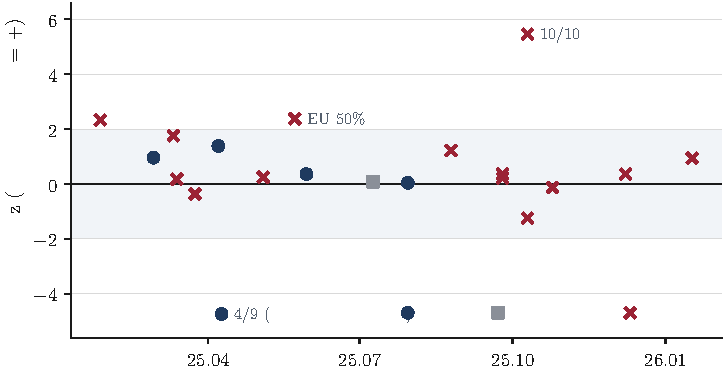
\includegraphics[width=\linewidth]{fig/res_esc_scatter.pdf}
\end{column}
\begin{column}{0.38\textwidth}
\begin{itemize}
\item 강화 위협 20건 중 16건이 위험회피 방향 (부호검정 $p=0.012$)
\item 평균 $z=0.59$, 중앙값 $0.36$
\item S\&P 500의 30분 반응 중앙값은 $-0.09\%$
\item 큰 반응은 소수: 10/10 대중 위협, EU 50\%
\end{itemize}
\end{column}
\end{columns}
\end{frame}

\begin{frame}{결과 2: 시간에 따른 변화}
\msg{시간이 지나도 반응은 줄지 않았다}
\begingroup\tfs
\begin{tabularx}{\textwidth}{@{}L{0.36\textwidth}rrrY@{}}
\toprule
비교 & 건수 & 평균 $z$ & 차이 & 검정\\
\midrule
전반 10건 (2025.1--5) & 10 & $0.45$ & & \\
후반 10건 (2025.7--2026.1) & 10 & $0.73$ & $-0.28$ & 순열 $p=0.74$\\
\addlinespace[2pt]
4/9 혼합 사건 제외 (전반/후반) & 19 & $1.02$/$0.73$ & $+0.29$ & 순위합 $p=0.24$\\
시간과의 순위상관 & 20 & & $\rho=-0.17$ & $p=0.47$\\
\bottomrule
\end{tabularx}\endgroup
\vspace{2mm}
\begin{itemize}
\item 과거 위협의 실행률에 대한 기울기 회귀도 0과 구분되지 않는다 ($b=5.5$, 표준오차 $6.8$)
\item 다만 이 회귀는 검출 가능한 최소 기울기가 $28$로, 사실상 검정력이 없다
\end{itemize}
\takeaway{``위협이 쌓일수록 시장이 무뎌졌다''는 증거는 없다. 단, 전후반 차이의 표준오차가 $0.86$이라 $z$ 기준 $2.4$보다 작은 변화는 이 표본으로 검출할 수 없다.}
\end{frame}

\begin{frame}{결과 3: 실행 여부별 반응}
\msg{시장은 실행될 위협과 아닌 위협을 구분하지 못했다}
\begin{columns}[c,onlytextwidth]
\begin{column}{0.5\textwidth}
\begingroup\tf
\begin{tabularx}{\linewidth}{@{}Yrr@{}}
\toprule
사후 결과 & 건수 & 발표 시점 평균 $z$\\
\midrule
실행·부분 실행 & 6 & $-0.32$\\
\quad 4/9 혼합 사건 제외 & 5 & $0.57$\\
미실행 & 14 & $0.98$\\
\bottomrule
\end{tabularx}\endgroup
\vspace{2mm}
{\small\RaggedRight 차이의 순열 검정 $p=0.19$, 혼합 사건을 빼면 순위합 $p=0.82$.\par}
\end{column}
\begin{column}{0.46\textwidth}
\begin{itemize}
\item 나중에 실행된 위협이 발표 때 더 크게 움직였다는 증거가 없다
\item 가장 큰 반응 두 건(10/10 대중 위협, EU 50\%)은 모두 \textbf{실행되지 않았다}
\end{itemize}
\end{column}
\end{columns}
\takeaway{실행된 인도 25\%, 구리 50\%는 발표 때 거의 무반응이었다. 실행 집단이 5--6건이라 이 비교의 검정력은 낮다.}
\end{frame}

\begin{frame}{결과 4: 철회와 발효}
\msg{철회에는 반응하고, 발효일에는 반응하지 않는다}
\begin{columns}[c,onlytextwidth]
\begin{column}{0.5\textwidth}
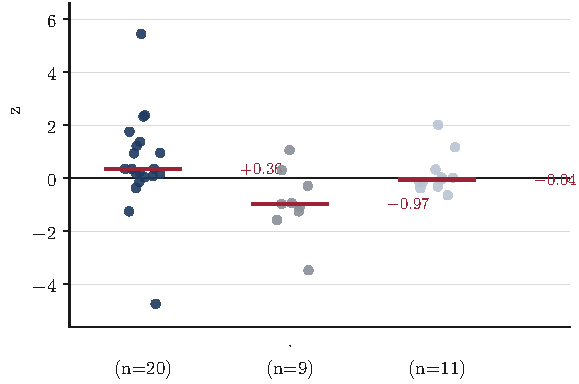
\includegraphics[width=\linewidth]{fig/res_groups.pdf}
\end{column}
\begin{column}{0.46\textwidth}
\begin{itemize}
\item \textbf{완화·철회} 9건: 평균 $z=-0.91$ ($t=-2.15$), 7건이 안도 방향. S\&P 500 중앙값 $+0.44\%$
\item \textbf{예정 발효} 11건: 평균 $z=0.17$ ($t=0.74$), 방향도 반반. S\&P 500 중앙값 $0.00\%$
\item 발효의 $|z|$는 발표보다 작다 (통화 기준 $p=0.03$)
\end{itemize}
\end{column}
\end{columns}
\end{frame}

\begin{frame}{사례: 10월 10일의 분 단위 경로}
\msg{가장 크게 움직인 위협이 실행되지 않은 위협이었다}
\begin{columns}[c,onlytextwidth]
\begin{column}{0.52\textwidth}
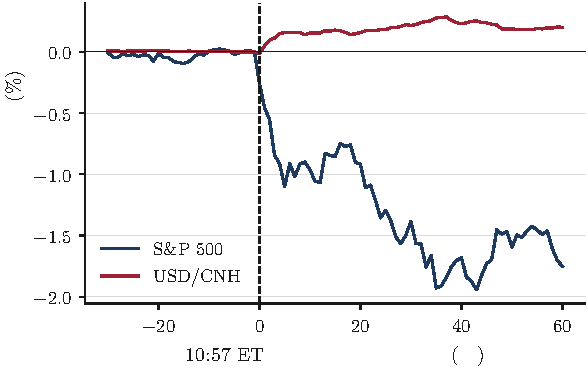
\includegraphics[width=\linewidth]{fig/res_oct10_min.pdf}
\end{column}
\begin{column}{0.44\textwidth}
\begin{itemize}
\item 게시 후 1분 안에 S\&P 500이 꺾이고, 위안화는 3분 뒤부터 약세
\item 35분 동안 S\&P 500 $-1.5\%$, USD/CNH $+0.22\%$
\item 표준화 반응 $z=5.5$로 표본 중 최대
\item 시간봉으로 본 두 번째 시도의 결론이 분 단위에서 확인된다
\end{itemize}
\end{column}
\end{columns}
\src{Dukascopy 1분봉(S\&P 500 CFD, USD/CNH). 이 사건은 설계 전에 이미 본 사건이라 주 결과는 이를 제외한 표본에서도 보고한다(평균 $z=0.42$, 18건).}
\end{frame}

\begin{frame}{강건성}
\msg{창, 표본, 정의를 바꿔도 부호는 같다}
\begingroup\tfs
\begin{tabularx}{\textwidth}{@{}L{0.34\textwidth}rrrY@{}}
\toprule
명세 & 강화 평균 $z$ (건수) & 완화 평균 $z$ & 발효 평균 $z$ & 비고\\
\midrule
주 명세 [$-5$, $+30$]분 & $0.59$ (20) & $-0.91$ & $0.17$ & \\
창 [$-5$, $+15$]분 & $0.83$ (20) & $-0.76$ & $0.11$ & 짧을수록 큼\\
창 [$-5$, $+60$]분 & $0.47$ (20) & $-0.80$ & $0.18$ & \\
창 [$-5$, $+120$]분 & $0.37$ (20) & $-0.43$ & $0.12$ & 길수록 희석\\
사전 열람 사건(10/10) 제외 & $0.42$ (18) & $-0.90$ & $0.17$ & \\
휴장 중 게시 제외 & $0.63$ (15) & $-1.07$ & $0.17$ & \\
2025.4.2--4.9 제외 & $0.84$ (18) & $-0.59$ & $0.28$ & 혼합 사건 제거\\
\bottomrule
\end{tabularx}\endgroup
\vspace{1.5mm}
\begin{itemize}
\item 부호는 모든 명세에서 같다: 강화 $+$, 완화 $-$, 발효 $\approx0$
\end{itemize}
\end{frame}

%================================================================
\section{해석}

\begin{frame}{해석 1: 미실행의 유형}
\msg{``미실행''은 한 종류가 아니다}
\begin{columns}[c,onlytextwidth]
\begin{column}{0.54\textwidth}
\begingroup\tf
\begin{tabularx}{\linewidth}{@{}Yrr@{}}
\toprule
위협의 결말 (사후 분류) & 건수 & 발표 시점 평균 $z$\\
\midrule
협상으로 낮춰 타결 & 4 & $1.88$\\
상대의 양보 & 4 & $1.15$\\
실제 실행 (4/9 제외) & 5 & $0.57$\\
일방적 보류·소멸 & 6 & $0.26$\\
\midrule
명시적으로 번복·합의 & 9 & $1.39$\\
시한만 지나 조용히 소멸 & 5 & $0.23$\\
\bottomrule
\end{tabularx}\endgroup
\vspace{1.5mm}
{\small\RaggedRight 협상·양보 대 일방 소멸: 순열 $p=0.16$. 명시 대 소멸: 순위합 $p=0.11$. 결과를 본 뒤의 분류다.\par}
\end{column}
\begin{column}{0.42\textwidth}
\begin{itemize}
\item 미실행 21건 중 9건은 상대의 양보나 협상 타결로 끝났다. 위협이 \textbf{통한} 경우다
\item 10건은 번복 발표도 없이 사라졌다. 시장은 이 위협들을 발표 때부터 거의 무시했다
\item 가장 크게 반응한 위협이 실행되지 않았다
\end{itemize}
\end{column}
\end{columns}
\end{frame}

\begin{frame}{해석 2: 반응의 경로와 지속성}
\msg{위협은 환율에, 철회는 주가에 실린다. 대부분 며칠 안에 지워진다}
\begin{columns}[t,onlytextwidth]
\begin{column}{0.47\textwidth}
\lab{어느 시장이 받는가}
\begingroup\tf
\begin{tabularx}{\linewidth}{@{}Yrr@{}}
\toprule
사건 & S\&P 평균 $z$ & 대상국 통화 평균 $z$\\
\midrule
강화 위협 & $0.43$ & $1.17$\\
완화·철회 & $-1.63$ & $-0.10$\\
발효 & $0.43$ & $-0.08$\\
\bottomrule
\end{tabularx}\endgroup
\vspace{1.5mm}
{\small\RaggedRight 위협은 특정 국가의 뉴스로 환율에, 철회는 미국 정책 불확실성의 해소로 주가에 실린다.\par}
\end{column}
\begin{column}{0.49\textwidth}
\lab{얼마나 남는가: 위협 뒤 S\&P 선물 (중앙값)}
\begingroup\tf
\begin{tabularx}{\linewidth}{@{}Yrrrr@{}}
\toprule
 & 30분 & 1일 & 3일 & 10일\\
\midrule
전체 19건 & $-0.11\%$ & $0.00\%$ & $+0.34\%$ & $+0.50\%$\\
\bottomrule
\end{tabularx}\endgroup
\vspace{1.5mm}
{\small\RaggedRight 예외는 큰 사건: 10/10 대중 위협은 하루 뒤 $-3.0\%$.\par}
\end{column}
\end{columns}
\vspace{1mm}
\begin{itemize}
\item 품목 관세는 지수가 아니라 해당 가격에 실린다: 구리 50\% 예고일에 미국 구리 선물은 $+12.4\%$, S\&P 반응은 $z=0.08$
\end{itemize}
\end{frame}

\begin{frame}{해석 3: 실행률의 기준과 두 경로}
\msg{낮은 실행률은 통상 위협의 일반적 성격이다. 큰 반응과 미실행은 함께 간다}
\begin{columns}[t,onlytextwidth]
\begin{column}{0.44\textwidth}
\lab{실행률은 원래 낮다}
\begingroup\tf
\begin{tabularx}{\linewidth}{@{}Yr@{}}
\toprule
자료 & 실행 비율\\
\midrule
제재 1,412건 (TIES) & 60\%\\
301조 91건 & 13\%\\
2기 (Bloomberg) & 약 25\%\\
본 연구 32건 & 22--34\%\\
\bottomrule
\end{tabularx}\endgroup
\vspace{1.5mm}
{\small\RaggedRight 제재 문헌에서 위협 단계 종결의 절반은 상대의 양보다.\par}
\end{column}
\begin{column}{0.52\textwidth}
\lab{큰 반응과 미실행이 함께 가는 두 경로 (가설)}
\begin{itemize}
\item \textbf{협상 카드:} 주요 교역국을 향한 큰 위협은 처음부터 협상용이고, 시장은 실행 확률이 아니라 판돈에 반응한다
\item \textbf{시장이 부른 후퇴:} 가격이 크게 흔들리면 발표자가 물러난다 (4월 9일 유예, 그린란드)
\end{itemize}
{\small\RaggedRight 이 자료로는 둘을 가를 수 없다.\par}
\end{column}
\end{columns}
\takeaway{발표효과에 필요한 것은 실행 실적이 아니라 실행 능력과 판의 크기다.}
\end{frame}

\begin{frame}{해석 4: 예측시장의 실행 확률}
\msg{시장은 실행 확률을 0.4 안팎으로, 대체로 맞게 매겼다}
\begin{columns}[c,onlytextwidth]
\begin{column}{0.47\textwidth}
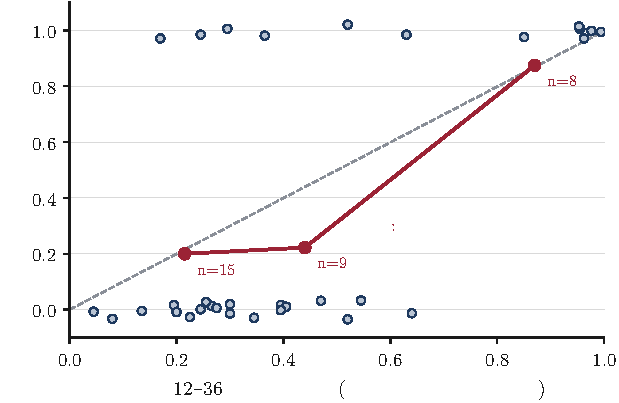
\includegraphics[width=\linewidth]{fig/pm_calib_s.pdf}
\end{column}
\begin{column}{0.5\textwidth}
\begingroup\tf
\begin{tabularx}{\linewidth}{@{}Yrrr@{}}
\toprule
가격 구간 & 계약 & 평균 가격 & 실행 비율\\
\midrule
0.30 이하 & 15 & $0.22$ & $0.20$\\
0.30--0.60 & 9 & $0.44$ & $0.22$\\
0.60 초과 & 8 & $0.87$ & $0.88$\\
\midrule
전체 & 32 & $0.44$ & $0.38$\\
\bottomrule
\end{tabularx}\endgroup
\vspace{1.5mm}
\begin{itemize}
\item Polymarket의 발효 여부 계약 32건
\item 실행된 계약의 가격이 더 높았다 (순위합 $p=0.008$)
\end{itemize}
\end{column}
\end{columns}
\end{frame}

\begin{frame}{해석 5: 사건 시점의 믿음 변화}
\msg{위협은 믿음을 올리고, 철회는 남은 믿음을 지운다}
\begin{columns}[c,onlytextwidth]
\begin{column}{0.64\textwidth}
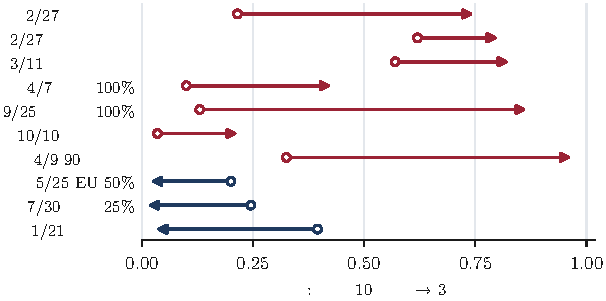
\includegraphics[width=\linewidth]{fig/pm_jumps_s.pdf}
\end{column}
\begin{column}{0.33\textwidth}
\begin{itemize}
\item 위협은 계약 가격을 19--75\%p 올렸다
\item 철회 직전의 가격은 0.20--0.40. 시장은 번복 전에 이미 낮게 보고 있었다
\item 의약품 100\%: 확률은 75\%p 뛰었지만 S\&P 반응은 $z=0.21$
\end{itemize}
\end{column}
\end{columns}
\takeaway{가격 반응이 작다고 믿지 않은 것은 아니다. 반응은 믿음의 변화에 손실의 크기를 곱한 값이다.}
\end{frame}

\begin{frame}{확장: 수출통제 예고와 상대 주가}
\msg{2025년 이후 통제 예고는 국산 대체 쪽으로, 번복은 반대로 가격을 옮겼다}
\begin{columns}[c,onlytextwidth]
\begin{column}{0.56\textwidth}
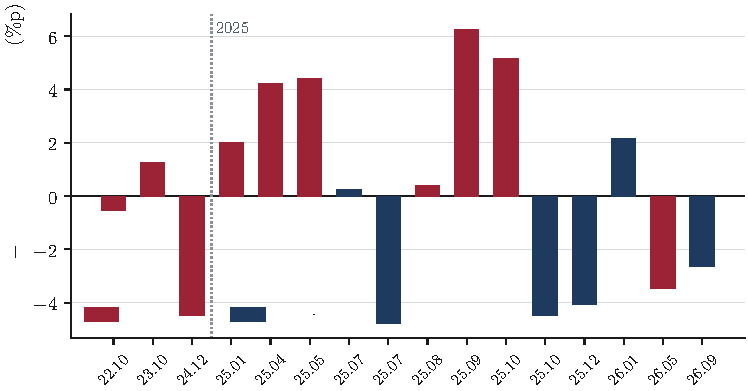
\includegraphics[width=\linewidth]{fig/xc_spread.pdf}
\end{column}
\begin{column}{0.41\textwidth}
\begingroup\tf
\begin{tabularx}{\linewidth}{@{}Yrr@{}}
\toprule
사건 다음 거래일 & 건수 & 상대수익\\
\midrule
강화, 2022--24 & 3 & $-1.24$\\
강화, 2025 이후 & 7 & $+2.71$\\
완화·번복 & 6 & $-2.25$\\
\bottomrule
\end{tabularx}\endgroup
\vspace{1.5mm}
{\small\RaggedRight 상대수익: 중국 국산 대체 12개사 $-$ 미국 공급사 10개사 초과수익(\%p). 2025년 이후 강화 대 완화의 순위합 $p=0.022$.\par}
\end{column}
\end{columns}
\begin{itemize}
\item 수출통제 사건 17건 중 강화 10건, 그 절반이 나중에 번복되거나 실행되지 않았다
\end{itemize}
\end{frame}

\begin{frame}{결론}
\msg{시장은 위협을 믿거나 안 믿는 것이 아니라, 가려 듣는다}
\begin{itemize}
\item \textbf{말뿐인 위협도 시장을 움직인다.} 20건 중 16건이 위험회피 방향, 2년간 줄지 않았다
\item \textbf{반응은 판의 크기를 따른다.} 실행 여부가 아니라 협상의 대상이 될 만한 위협에 크게 반응했다
\item \textbf{실행률은 신뢰도가 아니다.} 예측시장은 실행 확률을 0.4 안팎으로 맞게 매겼다
\item \textbf{발효일은 사건이 아니다.} 정보는 말이 나오는 순간과 거둬지는 순간에 도착한다
\item \textbf{발표효과의 조건은 실행 실적이 아니라 실행 능력과 판의 크기다}
\end{itemize}
\vspace{1.5mm}
\begin{columns}[T,onlytextwidth]
\begin{column}{0.48\textwidth}
\lab{한계}
\begin{itemize}
\item 사건 40건. 집단 비교의 검정력이 낮다
\item 결말별 분류와 수출통제 분석은 사후적이다
\end{itemize}
\end{column}
\begin{column}{0.48\textwidth}
\lab{남은 질문}
\begin{itemize}
\item 예고만으로 실제 연구개발 지출이 옮겨 갔는가
\item 2018--2019년에도 같은 구조였는가
\end{itemize}
\end{column}
\end{columns}
\end{frame}

%================================================================
\appendix
\section{부록}

\begin{frame}{부록 A. 게시 시각을 확인한 강화 위협 (일부)}
\begingroup\tfs\renewcommand{\arraystretch}{1.02}
\begin{tabularx}{\textwidth}{@{}llL{0.2\textwidth}L{0.28\textwidth}Y@{}}
\toprule
날짜 & ET & 대상 & 내용 & 결과\\
\midrule
2025-02-27 & 08:46 & 멕시코·캐나다·중국 & 3/4 예정대로, 중국 +10\% & 실행 (3/4)\\
2025-03-11 & 10:15 & 캐나다 철강 & 50\% & 미실행 (당일 번복)\\
2025-03-13 & 07:58 & EU 주류 & 200\% & 미실행\\
2025-04-07 & 11:14 & 중국 & +50\% & 실행 (4/9)\\
2025-05-23 & 07:43 & EU & 50\%, 6/1부터 & 미실행 (연기 후 15\% 합의)\\
2025-05-30 & 19:16 & 철강·알루미늄 & 50\%, 6/4부터 & 실행\\
2025-07-30 & 08:09 & 인도 & 25\%+벌칙 & 실행\\
2025-09-25 & 19:24 & 브랜드 의약품 & 100\%, 10/1부터 & 미실행 (보류)\\
2025-10-10 & 10:57 & 중국 & 대폭 인상 검토 & 미실행 (1년 연기)\\
2025-12-08 & 17:55 & 멕시코 & 5\% & 미실행 (12/12 철회)\\
2026-01-17 & 11:19 & 유럽 8국 & 10\%→25\% & 미실행 (1/21 철회)\\
\bottomrule
\end{tabularx}\endgroup
\end{frame}

\begin{frame}{부록 B. 10월 10일: 벤치마크와 과거 잔차}
\begin{columns}[c,onlytextwidth]
\begin{column}{0.48\textwidth}
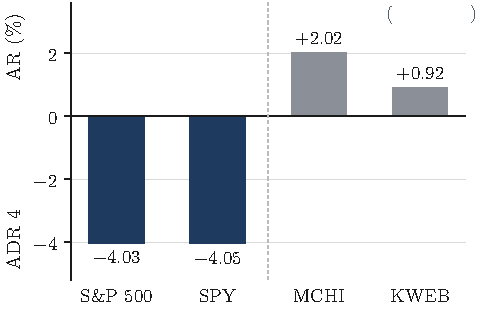
\includegraphics[width=\linewidth]{fig/s_fig_bench.pdf}
\end{column}
\begin{column}{0.5\textwidth}
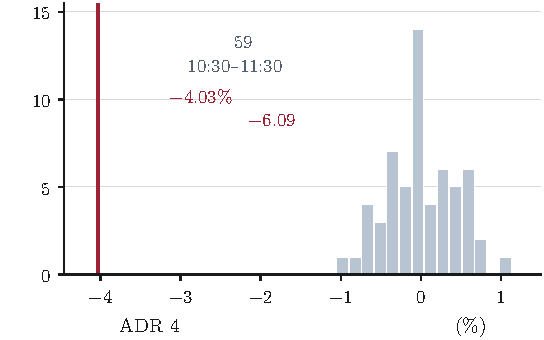
\includegraphics[width=\linewidth]{fig/s_fig_hist.pdf}
\end{column}
\end{columns}
\takeaway{중국 ETF를 기준으로 하면 ADR 4사의 상대 반응은 양수다. 표준화 예측오차 $-6.09$는 모형상 진단이며 정책 $p$값이 아니다.}
\end{frame}

\begin{frame}{참고문헌}
\linespread{1.0}
\begingroup\fontsize{7.3}{9.6}\selectfont\RaggedRight
\setlength{\parskip}{2.2pt}
\everypar{\hangindent=1.4em\hangafter=1}
Altavilla, C., Giannone, D., \& Lenza, M. (2016). The Financial and Macroeconomic Effects of the OMT Announcements. \textit{International Journal of Central Banking}, 12(3).\par
Amiti, M., Gomez, M., Kong, S. H., \& Weinstein, D. (2026 개정). Trade Protection, Stock-Market Returns, and Welfare. NBER WP 28758.\par
Gürkaynak, R. S., Sack, B., \& Swanson, E. (2005). Do Actions Speak Louder Than Words? \textit{International Journal of Central Banking}, 1(1).\par
Haddad, V., Moreira, A., \& Muir, T. (2021). When Selling Becomes Viral: Disruptions in Debt Markets in the COVID-19 Crisis and the Fed's Response. \textit{Review of Financial Studies}, 34(11), 5309--5351.\par
\endgroup
\end{frame}

\begin{frame}{참고문헌 (계속)}
\linespread{1.0}
\begingroup\fontsize{7.3}{9.6}\selectfont\RaggedRight
\setlength{\parskip}{2.2pt}
\everypar{\hangindent=1.4em\hangafter=1}
Kalemli-Özcan, Ṣ., Soylu, C., \& Yildirim, M. A. (2026). Tariff Uncertainty and the U.S. Dollar. NBER WP 34728.\par
Krishnamurthy, A., \& Vissing-Jorgensen, A. (2011). The Effects of Quantitative Easing on Interest Rates. \textit{Brookings Papers on Economic Activity}, Fall.\par
Merendino, A., \& Monacelli, T. (2026). Tariffs, Uncertainty, and the Exchange Rate. \textit{Economic Policy}, 게재예정.\par
Yale Program on Financial Stability. United States: Primary Market Corporate Credit Facility and Secondary Market Corporate Credit Facility.\par
자료: American Presidency Project(Truth Social 기록), PPAI/Thorn Run 관세 추적(2026 여름), Reuters 연표, Dukascopy, Yahoo Finance, Polymarket, Kalshi, EPO PATSTAT.\par
\endgroup
\end{frame}

\end{document}
